\documentclass[11pt,a4paper]{article}

% ---------- Font & ngôn ngữ ----------
\usepackage{fontspec}
\usepackage{polyglossia}
\setmainlanguage{vietnamese}

% ---------- Bố cục & định dạng ----------
\usepackage{geometry}
\geometry{a4paper, margin=2.5cm}
\usepackage{amsmath}
\usepackage{amssymb}
\usepackage{booktabs}
\usepackage{graphicx}
\usepackage{float}
\usepackage{enumitem}
\usepackage{listings}
\usepackage{xcolor}
\usepackage[font=small,labelfont=bf]{caption}
\usepackage[colorlinks=true,linkcolor=blue!60!black,
            citecolor=blue!60!black,urlcolor=blue!60!black]{hyperref}

\lstset{
    basicstyle=\small\ttfamily,
    frame=single,
    breaklines=true,
    showstringspaces=false,
    commentstyle=\itshape
}

\setlength{\parskip}{0.4em}
\setlength{\parindent}{0pt}
\setlength{\emergencystretch}{3em}

\title{\textbf{SO SÁNH BỐN THUẬT TOÁN ĐIỀU KHIỂN ĐÈN GIAO THÔNG}\\[3pt]
\large Fixed-Time --- MaxPressure --- Q-Learning --- Deep Q-Learning\\[4pt]
\normalsize Trên nền tảng mô phỏng GAMA kết hợp PyTorch}
\author{}
\date{}

\begin{document}

\maketitle
\vspace{-3em}

Báo cáo này tổng hợp quá trình triển khai và kết quả đánh giá so sánh bốn kỹ thuật
điều khiển đèn tín hiệu tại một ngã tư bốn hướng mô phỏng trên nền tảng GAMA:
(i)~điều khiển thời gian cố định (\textbf{Fixed-Time}), (ii)~điều phối theo áp lực
tối đa (\textbf{MaxPressure}), (iii)~học tăng cường dạng bảng (\textbf{Q-Learning})
và (iv)~học tăng cường sâu (\textbf{Deep Q-Learning}). Việc đánh giá được thực hiện
trên sáu tiêu chí hiệu năng giao thông; mỗi thuật toán chạy năm lần độc lập với cùng
luồng sinh xe để bảo đảm tính công bằng và khả năng lặp lại.

% =====================================================================
\section{Cách triển khai}
% =====================================================================

\subsection{Nền tảng mô phỏng chung}

Cả bốn thuật toán được cài đặt trong bốn tệp GAML riêng biệt
(\texttt{Traffic/models/}\allowbreak\texttt{intersection-*.gaml}) nhưng cùng nạp một
tệp mô hình cơ sở dùng chung \texttt{Traffic/includes/}\allowbreak\texttt{collision\_\allowbreak avoidance.gaml}. Nhờ đó toàn bộ hạ tầng
mô phỏng --- mạng đường, logic di chuyển của xe, điểm sinh xe, cách tính chỉ số ---
đồng nhất tuyệt đối giữa bốn mô hình, chỉ khác nhau ở bộ điều khiển đèn:

\begin{itemize}[leftmargin=*]
    \item \textbf{Ngã tư bốn hướng}, mỗi chiều có 6 làn xe; bước mô phỏng 0,1~giây;
    14 đoạn đường gồm 4 đường tiếp cận, 8 cung rẽ trong ngã tư và 2 đường đi thẳng qua.
    \item \textbf{Xe mô phỏng} gồm hai loại: ô tô (40\%, dài 4,5~m, chiếm 2 làn,
    $25$--$40$~km/h) và xe máy (60\%, dài 2,5~m, chiếm 1 làn, $20$--$35$~km/h).
    Xe rời chọn tuyến theo xác suất 50\%~đi thẳng / 25\%~rẽ trái / 25\%~rẽ phải,
    di chuyển theo mô hình bám xe IDM (Intelligent Driver Model).
    \item \textbf{Lưu lượng bất đối xứng}: trục Bắc--Nam sinh 1 xe mỗi 15 chu kỳ
    (1,5~giây), trục Đông--Tây 1 xe mỗi 45 chu kỳ (4,5~giây) --- tạo tình huống
    kiểm thử khó cho bộ điều khiển.
    \item \textbf{Tín hiệu chia 4 pha toàn cục}: \texttt{global\_phase} $\in$
    \{NS-GREEN, NS-YELLOW, EW-GREEN, EW-YELLOW\}; bốn nút tiếp cận cùng đọc biến
    toàn cục này để hiển thị đèn.
    \item \textbf{Sáu chỉ số hiệu năng} được cập nhật mỗi chu kỳ và xuất ra stdout
    dưới dạng dòng \texttt{METRIC\_CSV} mỗi 10 chu kỳ: throughput, thời gian chờ
    trung bình, chiều dài hàng đợi (xe có tốc độ $<1$~km/h), tốc độ trung bình,
    thời gian hành trình trung bình và thời gian chờ tối đa. Mỗi lần chạy batch
    kéo dài 2000 chu kỳ (200~giây mô phỏng).
\end{itemize}

\subsection{Fixed-Time --- điều khiển thời gian cố định}

\textbf{Tệp cài đặt:} \texttt{intersection-fixed-time.gaml}. Đây là bộ điều khiển
baseline, hoàn toàn không quan sát trạng thái giao thông. Chu kỳ đèn gồm bốn pha
cố định $\left[30, 3, 30, 3\right]$~giây (xanh B--N $\rightarrow$ vàng $\rightarrow$
xanh Đ--T $\rightarrow$ vàng), lặp lại mỗi 66~giây. Bộ điều khiển chỉ là một
máy trạng thái đếm thời gian trong reflex \texttt{traffic\_light\_controller}:

\begin{lstlisting}[language=Java]
// reflex traffic_light_controller - moi buoc mo phong 0.1s
global_counter += step;
if (global_counter >= phase_durations[global_phase]) {
    global_counter = 0;                       // reset bo dem cua pha
    global_phase = (global_phase + 1) mod 4;  // chuyen pha ke tiep
}
// phase_durations = [30s, 3s, 30s, 3s] - khai bao tinh, khong doi
\end{lstlisting}

Cách triển khai này đơn giản, tất định và dễ cấu hình, nhưng vì thời lượng pha
không phụ thuộc lưu lượng nên trong điều kiện demand bất đối xứng (trục đông,
trục vắng) sẽ xuất hiện lãng phí thời gian xanh ở trục vắng và dồn ứ ở trục đông.

\subsection{MaxPressure --- điều phối theo áp lực tối đa}

\textbf{Tệp cài đặt:} \texttt{intersection-maxpressure.gaml}, theo thuật toán
Max-Pressure của Varaiya~\cite{varaiya2013}. Nguyên lý: mỗi trục (B--N và Đ--T)
có một ``áp lực'' bằng \emph{số xe đang trên các đường tiếp cận trừ số xe đang trên
các đường rời}; pha xanh luôn ưu tiên trục có áp lực lớn hơn. Các danh sách đường
vào/ra cho từng trục được nạp một lần vào biến toàn cục
(\texttt{ns\_incoming\_roads}, \texttt{ew\_outgoing\_roads},\dots) để việc đếm xe
trong reflex \texttt{maxpressure\_controller} chạy nhanh.

Bộ điều khiển chỉ ra quyết định trong pha xanh và bị ràng buộc bởi bốn ngưỡng an toàn:

\begin{itemize}[leftmargin=*]
    \item \texttt{min\_green\_time} $= 10$~s: thời gian xanh tối thiểu, tránh đổi
    pha quá sớm;
    \item \texttt{check\_interval} $= 5$~s: chu kỳ đánh giá áp lực;
    \item \texttt{max\_green\_time} $= 60$~s: buộc đổi pha (\texttt{force\_switch})
    để tránh bỏ đói trục kia (starvation);
    \item \texttt{yellow\_time} $= 3$~s: pha vàng chuyển tiếp cố định, không AI
    can thiệp.
\end{itemize}

Điểm cốt lõi của thuật toán là quy tắc trễ (hysteresis) với biên $\delta = 2{,}0$ xe:
pha xanh chỉ bị rút ngắn khi áp lực trục đối diện vượt trội \emph{đủ lớn}, nhằm chống
hiện tượng dao động pha (anti-flicker) khi hai trục cân bằng:

\begin{equation}
P_{\text{NS}} = N^{\text{in}}_{\text{NS}} - N^{\text{out}}_{\text{NS}},
\qquad
P_{\text{EW}} = N^{\text{in}}_{\text{EW}} - N^{\text{out}}_{\text{EW}},
\qquad
\text{đổi pha} \iff P_{\text{đối diện}} > P_{\text{hiện tại}} + \delta .
\label{eq:maxpressure}
\end{equation}

\begin{lstlisting}[language=Java]
// Reflex maxpressure_controller - chi danh gia trong PHA XANH
check_now    = (phase_timer >= min_green) and (mod 5s tick);
force_switch = (phase_timer >= max_green);
if (check_now or force_switch) {
    // Dem xe theo duong hien tai cua tung xe
    pressure_NS = in_NS - out_NS;
    pressure_EW = in_EW - out_EW;
    if (global_phase == NS_GREEN and (force_switch
            or pressure_EW > pressure_NS + 2.0)) {
        global_phase = NS_YELLOW;   // chuyen tiep qua pha vàng 3s
    }
    // ... doi xung cho pha EW_GREEN
}
\end{lstlisting}

\textbf{Lỗi đã gặp và sửa:} khi chạy headless, phần \texttt{init} của mô hình thực
thi \emph{trước} khi mạng đường được tạo, khiến \texttt{intersection(1)} $=$ nil và
các danh sách đường rỗng $\Rightarrow$ áp suất luôn bằng 0, bộ điều khiển ``mù'' và
chỉ còn hành vi force-switch mỗi 60~giây. Khắc phục: chuyển việc nạp danh sách đường
sang reflex khởi tạo muộn \texttt{init\_road\_lists} (chạy khi
\texttt{length(intersection) > 3}), cách làm giống mô hình DQN.

\subsection{Q-Learning --- học tăng cường dạng bảng}

\textbf{Tệp cài đặt:} \texttt{intersection-qlearning.gaml}. Bộ điều khiển là một
agent học tăng cường~\cite{watkins1992} với bảng Q lưu trong biến
\texttt{map<string, list<float>> q\_table}. Không gian được rời rạc hóa như sau:

\begin{itemize}[leftmargin=*]
    \item \textbf{Trạng thái} (18 trạng thái $= 2 \times 3 \times 3$): pha xanh
    hiện tại $\in \{\text{NS}, \text{EW}\} \times$ mức hàng đợi trục B--N
    $\in \{0,1,2\} \times$ mức hàng đợi trục Đ--T $\in \{0,1,2\}$. Hàng đợi được
    phân cấp theo số xe đang dừng ($v < 1$~km/h) trên đường vào: $<5$ xe là mức 0,
    $5$--$14$ xe là mức 1, $\ge 15$ xe là mức 2. Mã hóa thành chuỗi
    ``\texttt{<pha>\_<muc NS>\_<muc EW>}'' làm khóa của bảng Q.
    \item \textbf{Hành động} (2): $0 = $ \textsc{Extend} (giữ pha xanh thêm) và
    $1 = $ \textsc{Switch} (chuyển sang pha vàng). Agent chỉ được hỏi mỗi 5~giây
    sau khi đã đạt thời gian xanh tối thiểu 10~giây; tại 60~giây buộc
    \textsc{Switch} để bảo đảm an toàn.
    \item \textbf{Thưởng} $r = -L$, với $L$ là tổng chiều dài hàng đợi hiện tại ---
    reward âm khuyến khích agent giải tỏa xe nhanh nhất có thể.
\end{itemize}

Sau mỗi lần quyết định, cặp (trạng thái trước, hành động trước) được cập nhật theo
phương trình Bellman dạng bảng với tốc độ học $\alpha = 0{,}1$ và hệ số chiết khấu
$\gamma = 0{,}9$:

\begin{equation}
Q(s,a) \leftarrow (1-\alpha)\,Q(s,a) + \alpha\Big(r + \gamma \max_{a'} Q(s',a')\Big).
\label{eq:bellman}
\end{equation}

Khám phá theo chiến lược $\varepsilon$-greedy: khởi tạo $\varepsilon_0 = 0{,}5$,
giảm $\varepsilon \leftarrow 0{,}995\,\varepsilon$ \emph{sau mỗi quyết định},
sàn $\varepsilon_{\min} = 0{,}05$; khi khai thác, chọn hành động có $Q$ lớn hơn
(nếu bằng nhau chọn ngẫu nhiên). Bảng Q được khởi tạo đầy đủ 18 trạng thái
$\times$ 2 hành động bằng 0 ngay trong \texttt{init} của mô hình.

\begin{lstlisting}[language=Java]
// Reflex qlearning_controller - tai moi diem quyet dinh (moi 5s)
curr_state = global_phase + "_" + level(queue_NS) + "_" + level(queue_EW);
// 1. Cap nhat Q cua buoc truoc (Bellman, reward = -tong hang doi)
old = Q[prev_state][prev_action];
Q[prev_state][prev_action] = (1-alpha)*old + alpha*(reward + gamma*max(Q[curr_state]));
// 2. Chon hanh dong theo epsilon-greedy
if (random() < epsilon) action = rnd(1);        // kham pha
else action = argmax(Q[curr_state]);            // khai thac
epsilon = max(eps_min, epsilon * 0.995);        // giam dan theo quyet dinh
// 3. Thuc thi: EXTEND -> giu xanh; SWITCH -> chuyen sang pha vang
\end{lstlisting}

Trong quá trình phát triển cũng phát hiện cùng lỗi headless như MaxPressure (danh
sách đường rỗng khi \texttt{init} chạy $\Rightarrow$ hàng đợi luôn bằng 0 $\Rightarrow$
không gian trạng thái suy biến), và được khắc phục bằng cùng cơ chế khởi tạo muộn.

\subsection{Deep Q-Learning --- học tăng cường sâu}

\textbf{Tệp cài đặt:} \texttt{intersection-dqn-python.gaml} (phía mô phỏng) và thư
mục \texttt{dqn\_py/} (phía Python/PyTorch): \texttt{gama\_env.py} (môi trường giao
thông dạng gym qua WebSocket), \texttt{dqn\_agent.py} (agent DQN), \texttt{train.py}
(vòng lặp huấn luyện), \texttt{evaluate.py} (đánh giá chính sách đã học).

\subsubsection*{Kiến trúc hai tiến trình}

Khác với Q-Learning bảng, DQN cần bộ xấp xỉ hàm bằng mạng nơ-ron; do đó hệ thống được
tách thành hai tiến trình giao tiếp qua \textbf{gama-server} (WebSocket, giao thức
JSON, thư viện chính thức \texttt{gama-client}, cổng 6868):

\begin{itemize}[leftmargin=*]
    \item \textbf{GAMA} giữ toàn bộ logic thời gian và an toàn \emph{giống hệt}
    mô hình Q-Learning bảng (xanh tối thiểu 10~s, tối đa 60~s, vàng 3~s, quyết định
    mỗi 5~s) để bảo đảm so sánh công bằng; nó cũng quan sát trạng thái
    (\texttt{queue\_ns}, \texttt{queue\_ew}, \texttt{approach\_ns},
    \texttt{approach\_ew} --- phân biệt xe đang dừng và xe đang chạy tới), xuất
    gói trạng thái và thực thi hành động của Python.
    \item \textbf{Python} chạy mạng DQN, nhận trạng thái, chọn hành động
    ($0=$ \textsc{Extend}, $1=$ \textsc{Switch}) và huấn luyện theo kinh nghiệm.
\end{itemize}

Tại mỗi điểm quyết định, hai bên bắt tay (handshake) theo năm bước:

\begin{lstlisting}[language=Python]
# Python (evaluate.py / train.py)  <->  GAMA (reflex dqn_controller)
state = await env.read_state()            # 1. GET state_pack (18 truong, noi boi "|")
await env.set_action(action)              # 2. SET dqn_action (0/1)
await env.step_cycles(1)                  # 3. GAMA ap dung action trong 1 chu ky
nb = await env.get_next_decision_in()     # 4. Doc so chu ky den tick quyet dinh ke tiep
await env.step_cycles(nb)                 # 5. Chay dung den tick do (sync=True)
\end{lstlisting}

Phía GAMA, reflex \texttt{update\_schedule} tính trước
\texttt{next\_decision\_in\_cycles} (phần còn lại của pha vàng $+$ thời gian xanh tối
thiểu, hoặc khoảng tick 5~giây kế tiếp trong pha xanh) giúp Python luôn bước mô phỏng
đúng đến điểm quyết định mà không bỏ sót tick.

\subsubsection*{Không gian trạng thái và mạng nơ-ron}

Trạng thái được nén thành \textbf{vector 8 chiều}, chuẩn hóa về $[0,1]$ bởi hàm
\texttt{featurize()} trong \texttt{gama\_env.py}:
\[
s = \Big[\tfrac{q_{\text{NS}}}{20},\ \tfrac{q_{\text{EW}}}{20},\
\tfrac{a_{\text{NS}}}{20},\ \tfrac{a_{\text{EW}}}{20},\
\tfrac{t_{\text{green}}}{600},\ \mathbb{1}[t_{\text{green}}\ge 100],\
\mathbb{1}[\text{pha NS}],\ \mathbb{1}[\text{pha EW}]\Big]
\]
trong đó $q$ là số xe đang dừng, $a$ là số xe đang tiến gần trên đường vào, và
$t_{\text{green}}$ là số chu kỳ đã trôi trong pha xanh hiện tại. Mạng $Q$ là MLP
$8 \rightarrow 32 \rightarrow 32 \rightarrow 2$ (ReLU), huấn luyện bằng bộ thành phần
chuẩn của DQN~\cite{mnih2015}: \emph{experience replay} (bộ đệm 20\,000 chuyển tiếp,
cấp phát trước bằng numpy), \emph{target network} đồng bộ mỗi 200 lần cập nhật, hàm
mất Huber trên minibatch 64 mẫu, kẹp gradient (max-norm 10) và tối ưu Adam với tốc độ
học $10^{-3}$. Target Bellman: $y = r + \gamma \max_{a'} Q_{\text{target}}(s',a')$
(với $y = r$ nếu kết thúc episode).

Reward và các siêu tham số học được đặt \emph{trùng khớp} với mô hình Q-Learning bảng
để so sánh công bằng: $r = -(w_q \cdot L_{\text{queue}} + w_w \cdot \bar{t}_{\text{wait}})$
với $(w_q, w_w) = (1{,}0;\, 0{,}0)$, $\gamma = 0{,}9$, $\varepsilon_0 = 0{,}5$,
$\varepsilon \leftarrow 0{,}995\,\varepsilon$ mỗi quyết định, $\varepsilon_{\min} = 0{,}05$.

\begin{table}[H]
\centering
\footnotesize
\setlength{\tabcolsep}{4.5pt}
\caption{So sánh cài đặt Q-Learning bảng và Deep Q-Learning}
\label{tab:hyperparams}
\begin{tabular}{lll}
\toprule
\textbf{Thành phần} & \textbf{Q-Learning bảng} & \textbf{Deep Q-Learning} \\
\midrule
Biểu diễn trạng thái & 18 trạng thái rời rạc & Vector 8 chiều $\in [0,1]^{8}$ \\
Bộ xấp xỉ $Q$ & Bảng \texttt{map<string, list>} & MLP $8{\to}32{\to}32{\to}2$ (PyTorch) \\
Hành động & \textsc{Extend} / \textsc{Switch} & Giống hệt bảng \\
Thưởng & $-L_{\text{queue}}$ & $-(w_q L + w_w \bar{t})$, $(w_q,w_w){=}(1{,}0;0{,}0)$ \\
$\gamma$ / lr & $0{,}9$ / $0{,}1$ (Bellman bảng) & $0{,}9$ / $10^{-3}$ (Adam) \\
Khám phá & $\varepsilon$-greedy $0{,}5{\to}\times0{,}995{\to}0{,}05$ & Giống hệt bảng \\
Kỹ thuật huấn luyện & Cập nhật ngay mỗi quyết định & Replay 20\,000, batch 64, target sync 200 \\
Nơi thực thi & Trong tiến trình GAMA & Python (MPS/CUDA/CPU) qua gama-server \\
\bottomrule
\end{tabular}
\end{table}

\subsubsection*{Huấn luyện, đánh giá và các sửa lỗi kỹ thuật}

\textbf{Huấn luyện} (\texttt{train.py}): 150 episode, mỗi episode 2000 chu kỳ
(200~giây), seed của episode $e$ là $1000 + e$. Mỗi quyết định: featurize trạng thái
$\rightarrow$ chọn hành động $\varepsilon$-greedy $\rightarrow$ handshake với GAMA
$\rightarrow$ lưu chuyển tiếp $(s, a, r, s', done)$ vào replay $\rightarrow$ một bước
gradient trên minibatch. Trọng số tốt nhất theo reward episode cao nhất được lưu vào
\texttt{best\_weights.pt}, kèm checkpoint định kỳ và nhật ký
\texttt{training\_log.csv}.

\textbf{Đánh giá} (\texttt{evaluate.py}): chạy lại mô phỏng với chính sách tham lam
thuần ($\varepsilon = 0$) sử dụng \texttt{best\_weights.pt} đã huấn luyện, ghi kết quả
ra \texttt{dqn\_metrics.csv} cùng schema với dòng \texttt{METRIC\_CSV} của ba mô hình
kia để ghép thẳng vào pipeline so sánh.

Hai lỗi kỹ thuật đáng chú ý đã được xử lý trong quá trình triển khai:

\begin{enumerate}[leftmargin=*]
    \item \textbf{Seed bị gama-server bỏ qua}: tham số đặc biệt \texttt{seed} truyền
    qua lệnh \texttt{reload} của gama-server không được áp dụng, khiến mọi episode
    chạy trùng nhau. Khắc phục bằng cách truyền seed như một tham số thường
    \texttt{rng\_seed}; mô hình GAMA tự gán \texttt{seed} trong \texttt{init} trước
    khi sinh xe.
    \item \textbf{Tick quyết định không tất định}: bộ đếm \texttt{phase\_timer} dạng
    float (bước 0,1~s) tích lũy sai số làm tròn, khiến các tick 10~s, 15~s,\dots{}
    lệch bất định. Mô hình DQN thay bằng bộ đếm nguyên
    \texttt{green\_cycles}/\texttt{yellow\_cycles} (ngưỡng 100/600/30/50 chu kỳ) ---
    tick quyết định hoàn toàn tất định trên lưới nguyên.
\end{enumerate}

% =====================================================================
\section{Kết quả benchmark và kết luận}
% =====================================================================

\subsection{Thiết lập thí nghiệm}

Benchmark được điều phối bởi script \texttt{scripts/compare\_4\_models.py} với tham
số \texttt{-{}-runs 5}, tức \textbf{mỗi thuật toán chạy 5 lần độc lập}, mỗi lần
2000 chu kỳ (200~giây mô phỏng):

\begin{itemize}[leftmargin=*]
    \item \textbf{Fixed-Time, MaxPressure, Q-Learning}: chạy batch headless bằng
    lệnh \texttt{gama-headless.sh -batch} \texttt{my\_batch\_experiment <model.gaml>}; GAMA
    tự chọn seed cho từng lần chạy (tạo nhiễu tự nhiên giữa các lần), stdout được
    đọc trực tiếp và bóc tách các dòng \texttt{METRIC\_CSV} (199 mẫu mỗi lần chạy,
    chu kỳ 10--1990).
    \item \textbf{Deep Q-Learning}: gama-server chạy sẵn ở cổng 6868;
    \texttt{evaluate.py} thực thi 5 episode với chính sách tham lam ($\varepsilon=0$)
    dùng trọng số tốt nhất đã huấn luyện (\texttt{best\_weights.pt} của lần chạy
    \texttt{train\_20260829\_153936}), seeds 5001--5005.
\end{itemize}

Với mỗi lần chạy, giá trị của sáu tiêu chí được quy đổi về một số: throughput và
thời gian hành trình lấy \emph{giá trị cuối}, thời gian chờ tối đa lấy \emph{giá trị
lớn nhất}, còn thời gian chờ trung bình / hàng đợi / tốc độ lấy \emph{trung bình theo
thời gian}. Bảng kết quả tổng hợp dạng mean~$\pm$~std trên 5 lần chạy; biểu đồ vẽ
series đại diện (lần chạy có throughput cuối ở vị trí median) của từng thuật toán.

\subsection{Kết quả tổng hợp}

\begin{table}[H]
\centering
\footnotesize
\setlength{\tabcolsep}{4pt}
\caption{Kết quả so sánh bốn thuật toán --- mean~$\pm$~std trên 5 lần chạy độc lập
(mỗi lần 2000 chu kỳ $=$ 200~giây). Throughput và tốc độ: cao hơn tốt hơn; các tiêu
chí còn lại: thấp hơn tốt hơn. DQL: Deep Q-Learning.}
\label{tab:ketqua}
\begin{tabular}{lccccl}
\toprule
\textbf{Tiêu chí} & \textbf{Fixed-Time} & \textbf{MaxPressure} & \textbf{Q-Learning} & \textbf{Deep Q-Learn.} & \textbf{Tốt nhất} \\
\midrule
1. Throughput (xe/200\,s)   & 111{,}20~$\pm$~1,94 & 109{,}40~$\pm$~2,87 & \textbf{111{,}80~$\pm$~4,26} & 110{,}40~$\pm$~3,14 & Q-Learning \\
2. Thời gian chờ TB (s)     & 5{,}24~$\pm$~0,44   & 3{,}63~$\pm$~0,31   & 3{,}81~$\pm$~0,37           & \textbf{2{,}05~$\pm$~0,10}   & DQL \\
3. Hàng đợi TB (xe)         & 6{,}18~$\pm$~0,52   & 4{,}61~$\pm$~0,40   & 4{,}95~$\pm$~0,43           & \textbf{2{,}69~$\pm$~0,12}   & DQL \\
4. Tốc độ TB (km/h)         & 17{,}29~$\pm$~0,44  & 18{,}56~$\pm$~0,29  & 18{,}20~$\pm$~0,16          & \textbf{19{,}74~$\pm$~0,23}  & DQL \\
5. Thời gian hành trình (s) & 47{,}69~$\pm$~1,26  & 45{,}16~$\pm$~0,53  & 46{,}13~$\pm$~0,75          & \textbf{43{,}43~$\pm$~0,56}  & DQL \\
6. Chờ tối đa (s)           & 36{,}54~$\pm$~1,52  & 31{,}50~$\pm$~4,67  & 28{,}78~$\pm$~2,71          & \textbf{16{,}26~$\pm$~0,94}  & DQL \\
\midrule
\multicolumn{6}{l}{\textit{Số tiêu chí thắng (theo mean): Fixed-Time: 0 \quad
MaxPressure: 0 \quad Q-Learning: 1 \quad Deep Q-Learning: 5}} \\
\bottomrule
\end{tabular}
\end{table}

\begin{figure}[H]
\centering
\makebox[\textwidth][c]{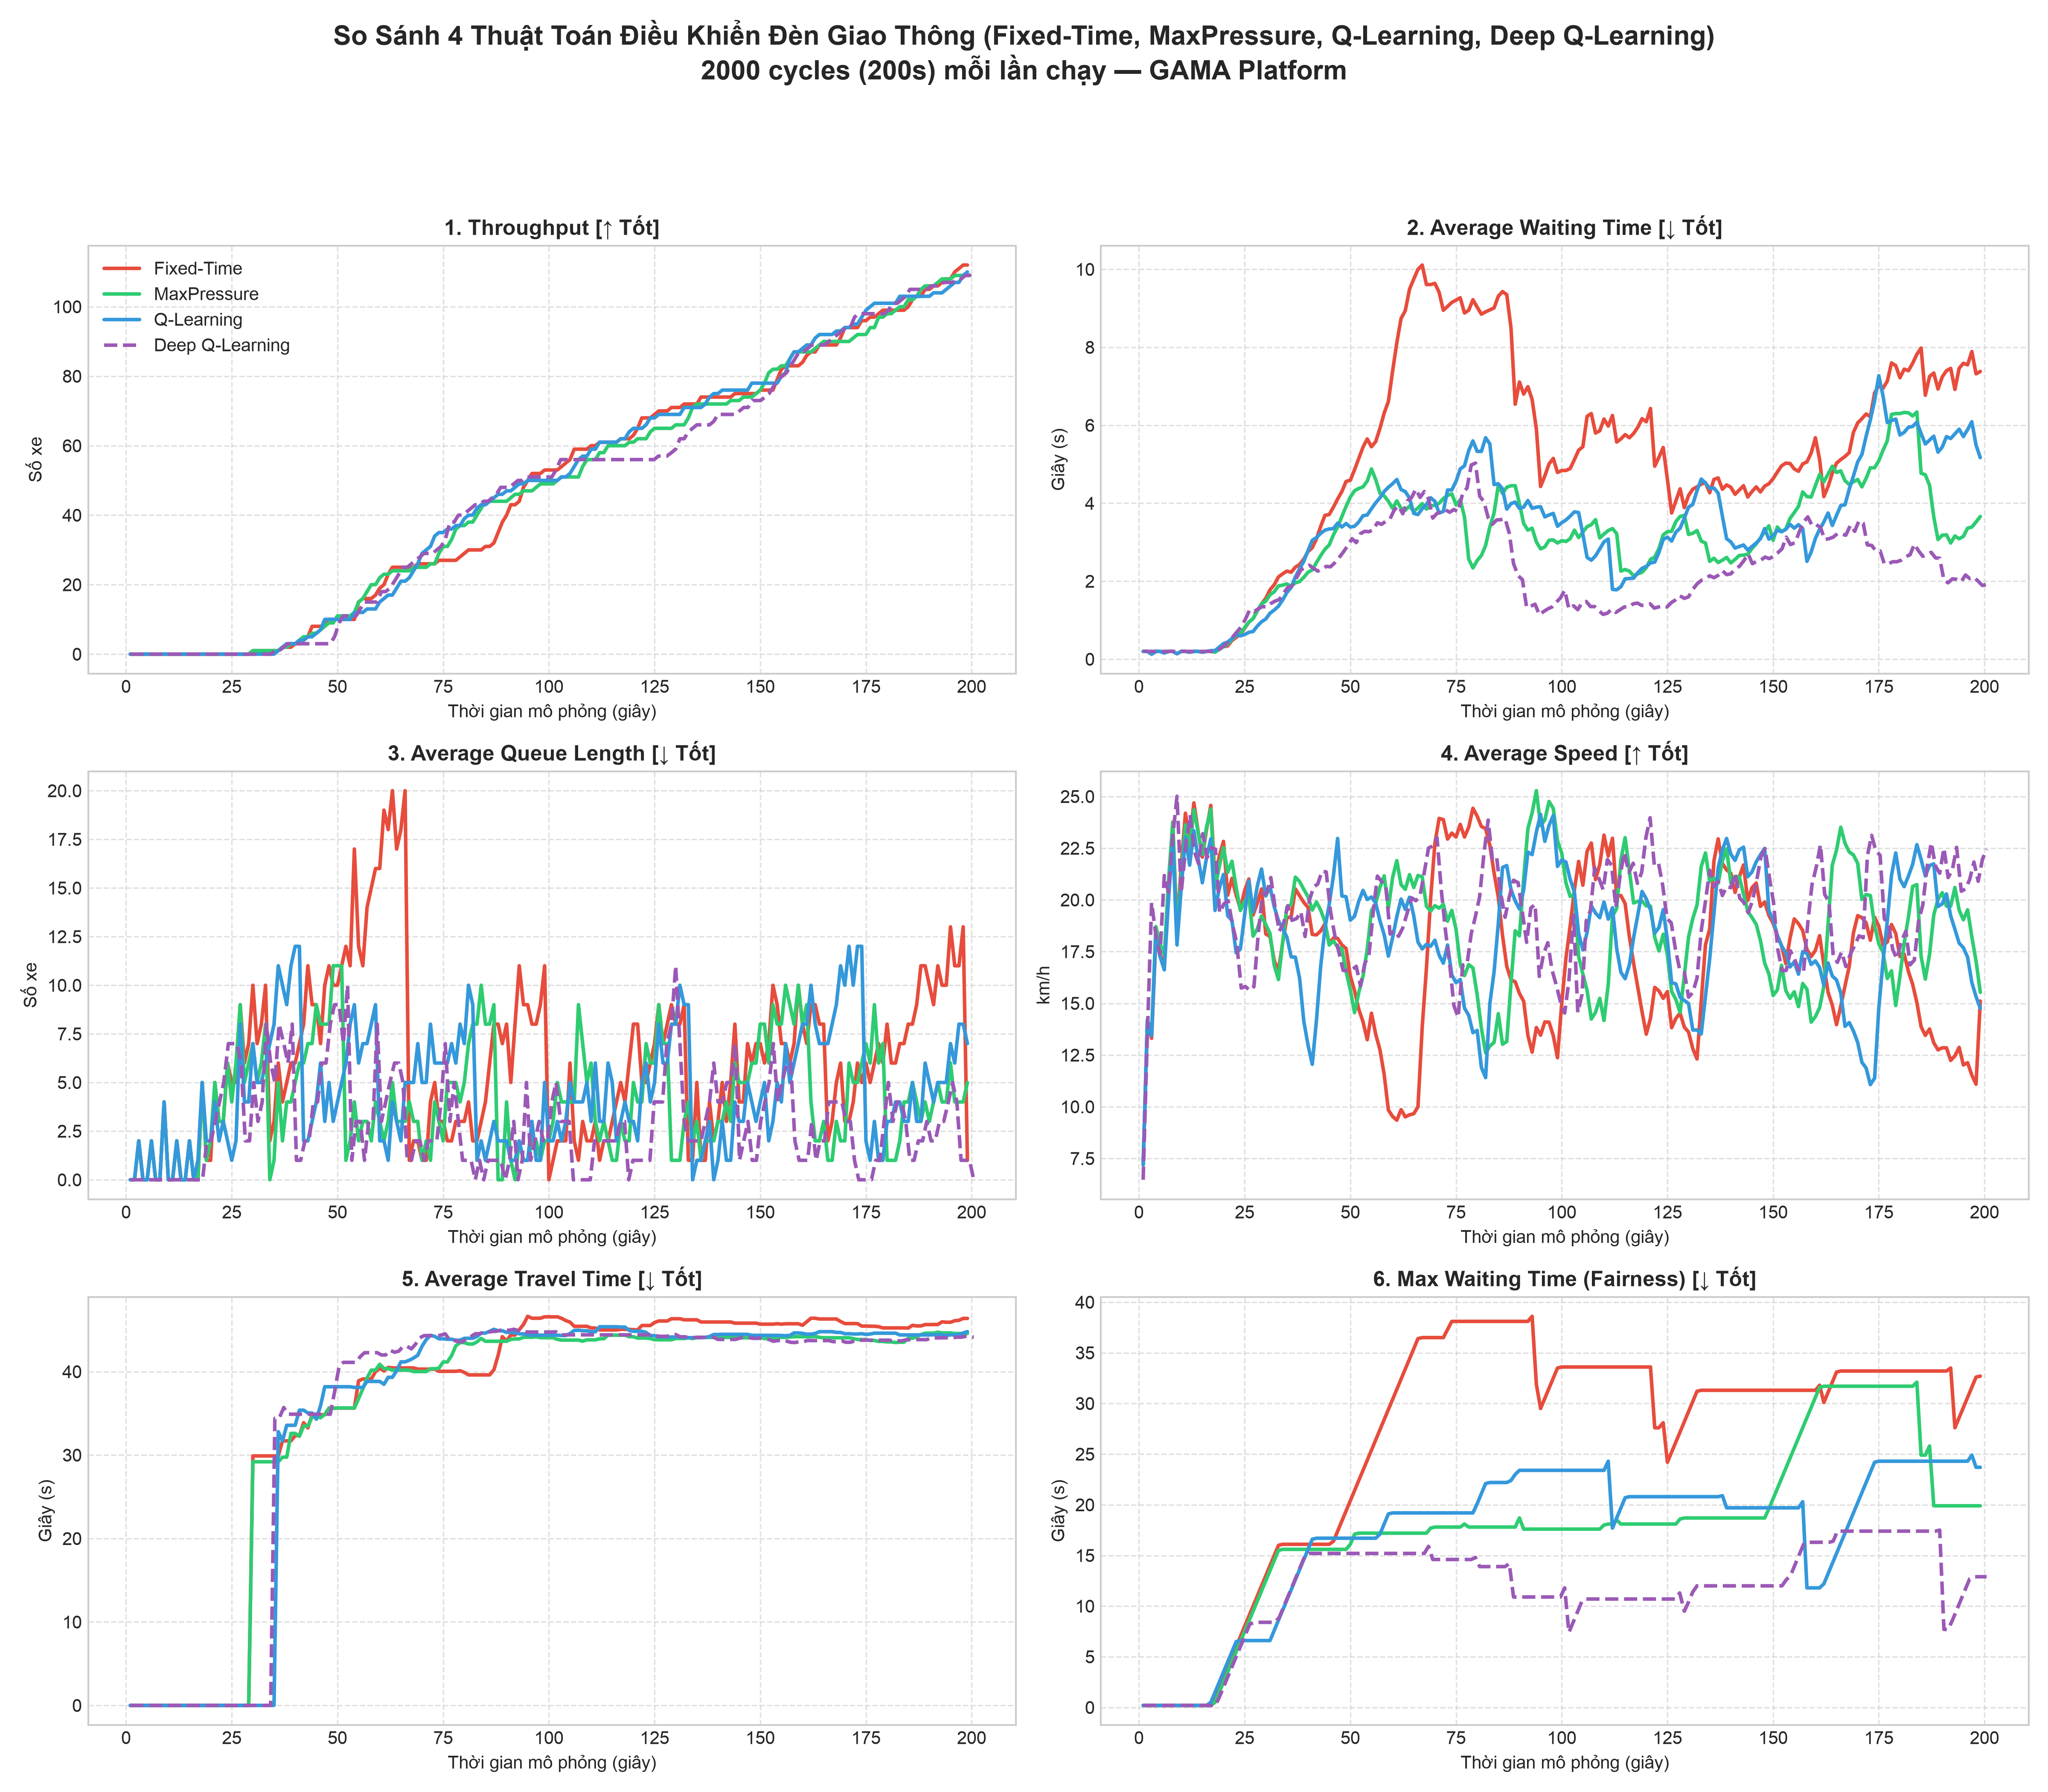
\includegraphics[width=1.15\textwidth]{../comparison_results/traffic_comparison_4models_6metrics.png}}
\caption{Diễn biến sáu tiêu chí theo thời gian mô phỏng (series đại diện, 200~giây):
Fixed-Time (đỏ), MaxPressure (xanh lá), Q-Learning (xanh dương), Deep Q-Learning
(tím, nét đứt).}
\label{fig:chart}
\end{figure}

\subsection{Phân tích kết quả}

\textbf{Throughput (tiêu chí 1).} Cả bốn thuật toán cho throughput gần nhau
($107$--$119$ xe/200~giây) và các đường throughput trong Hình~\ref{fig:chart} gần
như trùng nhau. Điều này dễ hiểu: luồng sinh xe là nút thắt của hệ thống, nên mọi
bộ điều khiển đều kịp giải tỏa toàn bộ demand. Khác biệt thật sự nằm ở \emph{chi
phí} phải trả để đạt được cùng lượng xe qua ngã tư.

\textbf{Chờ trung bình và hàng đợi (tiêu chí 2--3).} Fixed-Time tệ nhất với
5{,}24~giây chờ và 6{,}18 xe hàng đợi trung bình, với các đợt dồn ứ rõ rệt trên
biểu đồ (hàng đợi có lúc đạt đỉnh $\sim$20 xe, chờ trung bình đỉnh $\sim$10~giây)
trùng với lúc trục đông bị trì hoãn bởi chu kỳ cố định. Hai thuật toán thích ứng
giảm mạnh: MaxPressure 3{,}63~giây ($-31\%$), Q-Learning 3{,}81~giây ($-27\%$).
Deep Q-Learning tốt nhất với 2{,}05~giây ($-61\%$ so với Fixed-Time) và hàng đợi
2{,}69 xe ($-56\%$) --- nhờ mạng nơ-ron quan sát được cả lưu lượng \emph{đang tiến
gần} (approach), cho phép chủ động chuyển pha trước khi hàng đợi kịp hình thành.

\textbf{Tốc độ và thời gian hành trình (tiêu chí 4--5).} Thứ tự tương tự:
DQN đạt tốc độ trung bình cao nhất 19{,}74~km/h ($+14\%$ so với Fixed-Time) và
thời gian hành trình ngắn nhất 43{,}43~giây ($-9\%$). Ba đường travel time hội tụ
về gần nhau ở cuối mô phỏng, cho thấy advantage của RL chủ yếu nằm ở pha khởi động
khi demand đang tăng.

\textbf{Công bằng (tiêu chí 6).} Đây là tiêu chí chênh lệch rõ nhất: thời gian
chờ tối đa của Fixed-Time là 36{,}54~giây, của DQN chỉ còn 16{,}26~giây
($-55\%$). Đáng chú ý, DQN còn có độ lệch chuẩn nhỏ nhất (0{,}94) trên 5 lần chạy
--- chính sách học được không chỉ tốt hơn mà còn \emph{ổn định}; ngược lại
MaxPressure có std lớn (4{,}67) do chính sách nhạy theo tức thời của áp lực.

\textbf{Đánh giá chung.} Deep Q-Learning thắng 5/6 tiêu chí; Q-Learning bảng chỉ
thắng throughput (với std lớn nhất 4{,}26 --- kết quả dao động nhiều giữa các lần
chạy). MaxPressure tốt hơn Fixed-Time ở mọi tiêu chí còn lại, khẳng định giá trị
của điều khiển thích ứng. Thứ tự tổng thể: \textbf{Deep Q-Learning $>$ MaxPressure
$\approx$ Q-Learning $>$ Fixed-Time}.

\subsection{Kết luận và hướng phát triển}

Bốn bộ điều khiển đèn giao thông đã được triển khai hoàn chỉnh và đánh giá trên
cùng một nền tảng mô phỏng GAMA, cùng cấu hình ngã tư và cùng luồng sinh xe. Kết
luận chính:

\begin{itemize}[leftmargin=*]
    \item \textbf{Deep Q-Learning là phương pháp tốt nhất} trong thí nghiệm này:
    giảm 61\% thời gian chờ trung bình, 56\% hàng đợi, 55\% thời gian chờ tối đa
    và tăng 14\% tốc độ so với baseline Fixed-Time, đồng thời có phương sai nhỏ
    nhất giữa các lần chạy. Đánh đổi là hệ thống phức tạp hơn (huấn luyện trước
    với PyTorch, hạ tầng gama-server/WebSocket) và cần thời gian huấn luyện
    150 episode.
    \item \textbf{MaxPressure là lựa chọn thực dụng tốt}: không cần huấn luyện,
    cài đặt trong ~100 dòng GAML, hiệu năng chỉ thấp hơn DQN và cao hơn hẳn
    Fixed-Time --- phù hợp khi muốn triển khai nhanh, không cần hạ tầng học máy.
    \item \textbf{Q-Learning bảng học được chính sách tốt} trong không gian 18
    trạng thái nhỏ, nhưng bị giới hạn bởi việc rời rạc hóa trạng thái (mất thông
    tin về lưu lượng tiến gần) và nhiễu cao giữa các lần chạy.
    \item \textbf{Fixed-Time chịu ảnh hưởng nặng của demand bất đối xứng}: với
    chu kỳ 66~giây cứng, trục đông bị dồn ứ trong khi trục vắng lãng phí thời gian
    xanh, thể hiện qua cả ba tiêu chí chờ/hàng đợi/công bằng.
\end{itemize}

Các hướng phát triển tiếp theo: (i)~kiểm định thống kê chính thức (ví dụ kiểm định
Wilcoxon rank-sum) thay vì so sánh mean--std; (ii)~mở rộng sang mạng nhiều ngã tư
với multi-agent RL; (iii)~phát triển hàm thưởng (thêm trọng số thời gian chờ, độ
công bằng); (iv)~thử nghiệm demand biến động theo thời gian và demand bão hòa;
(v)~so sánh thêm với baseline Webster và các biến thể DQN (Double DQN, Dueling).

% =====================================================================
\begin{thebibliography}{9}
\bibitem{varaiya2013} P. Varaiya, ``Max pressure control of a network of
signalized intersections,'' \emph{Transportation Research Part C: Emerging
Technologies}, vol. 36, pp. 177--195, 2013.
\bibitem{watkins1992} C. J. C. H. Watkins and P. Dayan, ``Q-learning,''
\emph{Machine Learning}, vol. 8, no. 3--4, pp. 279--292, 1992.
\bibitem{mnih2015} V. Mnih \emph{et al.}, ``Human-level control through deep
reinforcement learning,'' \emph{Nature}, vol. 518, no. 7540, pp. 529--533, 2015.
\bibitem{treiber2000} M. Treiber, A. Hennecke, and D. Helbing, ``Congested
traffic states in empirical observations and microscopic simulations,''
\emph{Physical Review E}, vol. 62, no. 2, pp. 1805--1824, 2000.
\bibitem{gama2019} P. Taillandier \emph{et al.}, ``Building, composing and
experimenting complex spatial models with the GAMA platform,''
\emph{GeoInformatica}, vol. 23, no. 2, pp. 299--322, 2019.
\end{thebibliography}

\end{document}